% !TeX program = xelatex
% 编译：在 Paper 目录运行 latexmk -xelatex main.tex（或在仓库根目录运行 latexmk -cd -xelatex Paper/main.tex）。
\documentclass{mcmthesis}

% ===== 基本信息：在此修改年份、队号、题号和论文标题 =====
\newcommand{\ContestYear}{2026}
\newcommand{\TeamNumber}{000000} % 待替换为本次参赛队号
\newcommand{\ProblemLetter}{B}
\newcommand{\PaperTitle}{Holding the Green Line: Coupled Water--Cover Dynamics, Cohort Optimization, and Compound-Hazard Resilience}
\mcmsetup{
  tstyle=\color{red}\bfseries,
  tcn=\TeamNumber, problem=\ProblemLetter,
  sheet=true, titleinsheet=true, keywordsinsheet=true,
  titlepage=false, abstract=true
}
\renewcommand{\headset}{\ContestYear\\MCM/ICM\\Summary Sheet}
\title{\PaperTitle}

\usepackage{times}
\usepackage{indentfirst}
\usepackage{needspace,tikz,subcaption,float,placeins}
\usepackage{booktabs}
\usepackage{algorithm}
\usepackage[noend]{algpseudocode}
\algrenewcommand\algorithmicrequire{\textbf{Input:}}
\algrenewcommand\algorithmicensure{\textbf{Output:}}
% Wrapped algorithm lines keep their indent.
\makeatletter\newcommand{\AlgWrap}[1]{\parbox[t]{\dimexpr\linewidth-\ALG@thistlm\relax}{#1\strut}}\makeatother
\usetikzlibrary{arrows.meta,positioning,calc}
\usepackage{lastpage}
% 中英文文献库：XeLaTeX + BibTeX；正文使用 \cite{REF01} 等引用键。
\usepackage{xeCJK}
\setmainfont{texgyretermes-regular.otf}[BoldFont=texgyretermes-bold.otf,ItalicFont=texgyretermes-italic.otf,BoldItalicFont=texgyretermes-bolditalic.otf]
\setCJKmainfont{FandolSong-Regular.otf}[BoldFont=FandolSong-Bold.otf,ItalicFont=FandolKai-Regular.otf]
\setCJKsansfont{FandolHei-Regular.otf}[BoldFont=FandolHei-Bold.otf]
\setCJKmonofont{FandolFang-Regular.otf}
\usepackage[backend=bibtex,style=numeric,sorting=none,maxbibnames=3,giveninits=true]{biblatex}
\usepackage{xurl}
\addbibresource{bibliography/references.bib}
% 有 DOI 时不重复输出同一文献的网址。
\AtEveryBibitem{%
  \iffieldundef{doi}{}{\clearfield{url}}%
  \clearfield{urlyear}\clearfield{urlmonth}\clearfield{urlday}%
}
\graphicspath{{Figure/}{../Figures/M1/}{../Figures/M2/}{../Reports/M1/}{../Reports/M2/}}
\geometry{headheight=14pt}
\setlength{\emergencystretch}{1.2em}
\hypersetup{hidelinks,pdfauthor={},pdftitle={MCM/ICM Paper}}

% Shared colour palette for inline TikZ schematics and executive brief
% Shared colours for the TikZ schematics; same roles and hex values as
% Code/figures_matlab/paper_style.m (mycolor.space, base #1E5F74).
%   water (P, I, M, W-bar)  teal   | vegetation (V, r, d)  green
%   wind and sand (E, S)    brown  | highlight             orange
%   limits and caps         red dashed
\definecolor{pWater}{HTML}{1E5F74}
\definecolor{pWaterMid}{HTML}{659FB6}
\definecolor{pWaterLight}{HTML}{DCEBF1}
\definecolor{pTeal}{HTML}{00828C}
\definecolor{pVeg}{HTML}{2B633C}
\definecolor{pVegMid}{HTML}{4AC087}
\definecolor{pVegLight}{HTML}{E3F3E8}
\definecolor{pSand}{HTML}{8F7159}
\definecolor{pSandLight}{HTML}{FFEACE}
\definecolor{pAccent}{HTML}{F49431}
\definecolor{pPV}{HTML}{D47216}
\definecolor{pPVLight}{HTML}{FDF1E3}
\definecolor{pPlum}{HTML}{7A437F}
\definecolor{pPlumLight}{HTML}{F2EBF3}
\definecolor{pLimit}{HTML}{D03B3B}
\definecolor{pInk}{HTML}{1F2B33}
\definecolor{pAxis}{HTML}{344A53}
\definecolor{pGrey}{HTML}{97AFB9}
\definecolor{pGreyDark}{HTML}{647B84}
\definecolor{pGrid}{HTML}{E6EBED}


% 保留旧论文的符号表、公式分组和交替灰底表格工具。
\newcommand{\shade}{\rowcolor{gray!22}}
\newcommand{\modelvars}[1]{%
  \par\begingroup\small
  \setlength{\tabcolsep}{4pt}\renewcommand{\arraystretch}{1.10}
  \noindent\begin{tabularx}{\linewidth}{@{}>{\raggedright\arraybackslash}p{0.29\linewidth} >{\raggedright\arraybackslash}X@{}}
  \toprule\textbf{Symbol} & \textbf{Meaning} \\\midrule
  #1
  \bottomrule\end{tabularx}\par\endgroup
}
\newenvironment{modeleq}
  {\par\addvspace{0.4\baselineskip}\noindent\begin{minipage}{\linewidth}\setlength{\abovedisplayskip}{6pt}\setlength{\belowdisplayskip}{6pt}}
  {\end{minipage}\par\addvspace{0.4\baselineskip}}

% Bold run-in paragraph headings (template prints them plain).
\makeatletter
\renewcommand\paragraph{\@startsection{paragraph}{4}{\z@}{1.2ex \@plus .5ex}{-1em}{\normalfont\normalsize\bfseries}}
\makeatother

% Float pages start at the top instead of being vertically centred.
\makeatletter\setlength{\@fptop}{0pt}\makeatother

\begin{document}

% ===== 第一页：Summary Sheet（摘要不编入正文章节编号） =====
\begin{abstract}
\begin{keywords}
Taklamakan protective belt; Two-clock eco-hydrology; Cohort MILP; Agrivoltaic cross-subsidy; Compound-Poisson resilience; Discretised 2-D substochastic Markov chain
\end{keywords}
\end{abstract}
\hypersetup{pageanchor=false}
\maketitle
\hypersetup{pageanchor=true}

% ===== 第二页起：目录及正文 =====
\pagestyle{main}
\tableofcontents
\clearpage

\section{Introduction}
\subsection{Problem background}
Spanning roughly $337{,}600\,\text{km}^2$, the Taklamakan Desert is China's largest shifting-sand desert and one of the most hyper-arid basins on Earth. In November 2024, China completed spatial closure of a $3{,}046$\,km ``Green Sand-Blocking Protective Belt'' encircling the desert margin \cite{REF12}. Yet sand control is meticulous, long-term work rather than a one-off construction project: \emph{locking} the perimeter on a map does not automatically \emph{hold} it over decades. Operating the belt requires managing a tightly coupled, non-stationary system shaped by scarce seasonal water, finite multi-year funds, construction and maintenance labour, and stochastic natural disasters \cite{REF06} (\textbf{Table~\ref{tab:protection-factors}}).

\begin{table}[htbp]
  \centering
  \caption{Key factors and quantities in protective-belt management.}
  \label{tab:protection-factors}
  \begingroup\small
  \renewcommand{\arraystretch}{1.18}
  \begin{tabularx}{\linewidth}{@{}>{\raggedright\arraybackslash}p{0.17\linewidth}
    >{\raggedright\arraybackslash}p{0.37\linewidth}
    >{\raggedright\arraybackslash}X@{}}
    \toprule
    \textbf{Factor} & \textbf{Representative quantities} & \textbf{Role in belt protection} \\
    \midrule
    Water supply & Ecological replenishment volume ($\text{m}^3$/yr); monthly irrigation timing
      & Sustains root-zone soil moisture and vegetation growth under extreme evaporative demand. \\
    Funding & Total budget (CNY); allocation shares in construction, O\&M, and supporting PV
      & Sets newly treated belt scale, photovoltaic revenue capacity, and ongoing maintenance. \\
    Labour & Annual workforce input (person-days/yr); construction vs.\ upkeep split
      & Supports shrub planting, seasonal irrigation, panel installation, and stand upkeep. \\
    Disaster shocks & Drought probability; storm frequency ($\text{yr}^{-1}$) and fractional cover loss
      & Causes canopy defoliation/burial, shrinks canal supply, and tests biological recovery. \\
    \bottomrule
  \end{tabularx}
  \endgroup
\end{table}

\subsection{Problem restatement}
\begin{enumerate}
  \item \textbf{Establish a coupled dynamic model (Task 1).}
  Use public meteorological and remote-sensing observations to quantify \textbf{vegetation coverage},
  \textbf{effective root-zone soil moisture}, and their \textbf{interactions with wind and sand}.

  \item \textbf{Optimise construction and resource allocation (Task 2).}
  Make an explicit trade-off between ecological benefits and economic costs over a 15-year horizon under a fixed budget and resource caps. Optimise \textbf{annual newly treated area}, \textbf{age-scheduled water replenishment}, \textbf{investment allocation ratios} across construction, O\&M, and revenue-generating photovoltaics (PV), and \textbf{labour input}; test \textbf{investment sensitivity} and derive an \textbf{actionable process criterion}.

  \item \textbf{Assess resilience and long-term benefits (Task 3).}
  Embed \textbf{stochastic compound disasters} (sandstorms, extreme droughts, wind erosion, and sand burial) and \textbf{climate-driven baseline drift} into the post-construction belt. Quantify \textbf{resistance and post-shock recovery} alongside \textbf{long-term ecological trajectories}.

  \item \textbf{Deliver an actionable policy and public brief (Task 4).}
\end{enumerate}

\subsection{Our work}
\begin{figure}[H]\centering
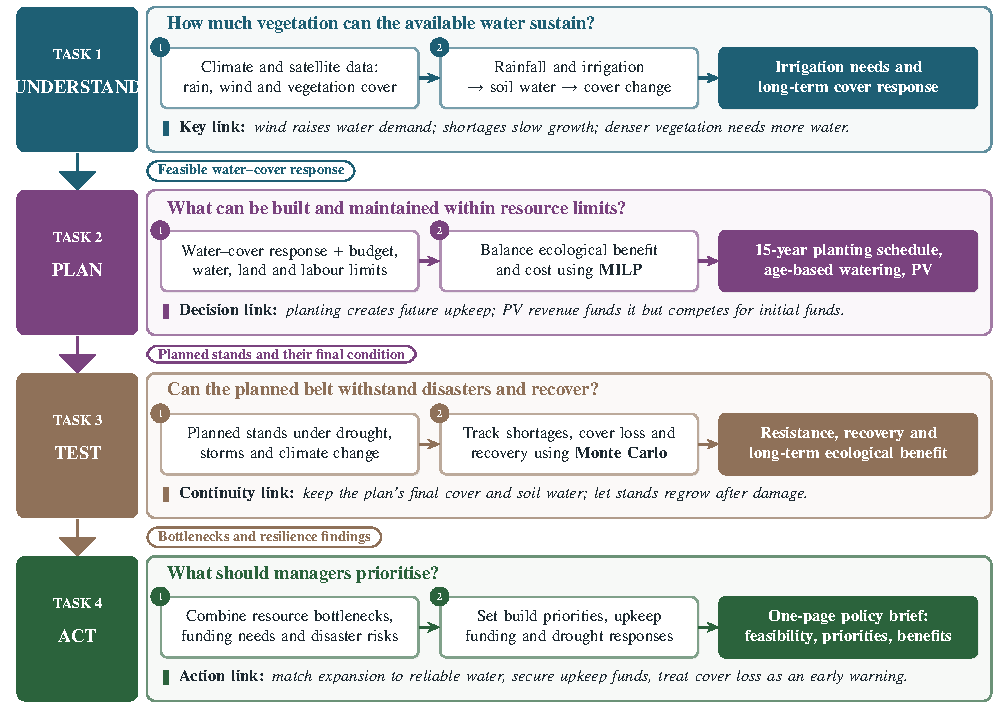
\includegraphics[width=0.9\linewidth]{workflow.pdf}
\caption{Overall workflow: understand, plan, test, and act.}\label{fig:framework}
\end{figure}

\subsection{Assumptions and Justifications}
\begingroup
\setlength{\topsep}{0pt}
\setlength{\partopsep}{0pt}
\setlength{\parsep}{0pt}
\setlength{\itemsep}{4pt}
\begin{enumerate}
  \item \textbf{Assumption:} \textbf{The reference section is locally uniform.} The Yutian--Minfeng section shares one climatic setting, and satellite-derived cover represents vegetation condition.
  \newline \textbf{Justification:} Public data cannot resolve variation within the narrow belt; conclusions apply to the reference section.

  \item \textbf{Assumption:} \textbf{Soil water changes daily and cover annually.} One root-zone store carries water between years; salinity feedback is omitted.
  \newline \textbf{Justification:} This captures short dry spells and slower vegetation growth with the available data. Omitting salinity may overstate long-term water benefits \cite{REF01,REF04}.

  \item \textbf{Assumption:} \textbf{Construction uses discrete lots and constant real unit costs.} New PV panels earn revenue from the following year.
  \newline \textbf{Justification:} Lot-based construction approximates field contracts, while fixed real prices keep multi-year costs comparable.

  \item \textbf{Assumption:} \textbf{Disaster risks follow declared scenarios.} During shortages, PV washing is supplied first and remaining water is shared proportionally among stands.
  \newline \textbf{Justification:} No local damage catalogue supports calibrated risk forecasts; the scenarios and allocation rule provide a consistent basis for conditional stress tests.
\end{enumerate}
\endgroup

\clearpage
\section{Data Collection and Preprocessing}\label{sec:data}
Our data answer one question: how much vegetation cover the desert margin can hold under the water and wind it receives. We build a station--month panel joining climate forcing with satellite-observed cover at nine sites around the Taklamakan, January 2015--December 2025 (9 stations $\times$ 132 months $=$ 1,188 station--months). Every record is fetched by script from a public archive.

\subsection{Study area and station categories}
The Taklamakan is ringed by river-fed oases, and the sand-locking belts we model lie on the boundary between these oases and the dune field \cite{REF06}. Stations sample this boundary on every side, plus two sites inside the desert (Figure~\ref{fig:data-stations}a). 1. \emph{Category~I (oasis margin)}: YT, MF, QM, RQ on the southern edge, KEL and YL on the lower Tarim River, ALE on the Aksu River; these calibrate Model~1, with YT--MF as the reference section. 2. \emph{Category~II (corridor)}: XT on the Desert Highway, whose shelterbelt survives only on saline drip irrigation \cite{REF01}. 3. \emph{Category~III (control)}: TZ in the desert centre. Categories II and III give context and are not fitted: margin sites hold 28--41\% cover, against about 1\% and 9\% (Figure~\ref{fig:data-stations}b), so pooling them would bias the fitted water--cover relation.

\begin{figure}[H]
  \centering
  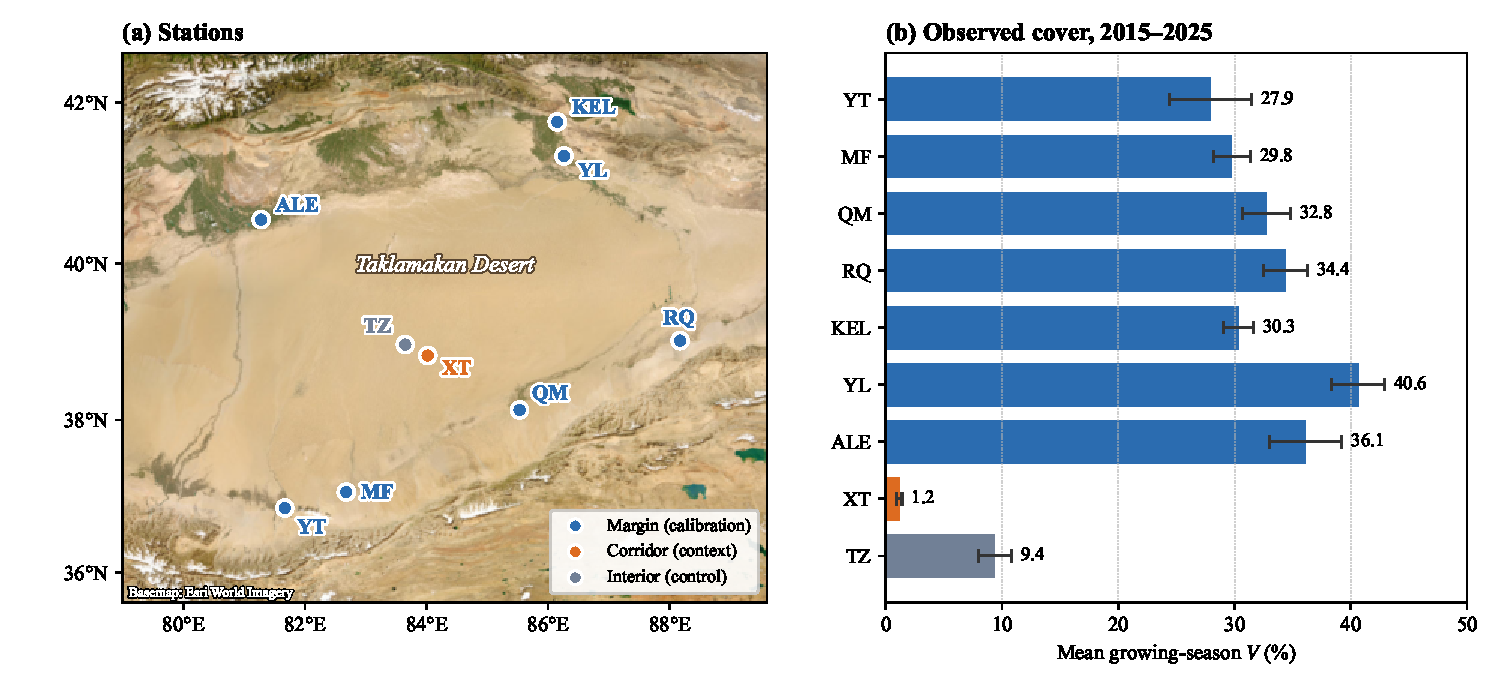
\includegraphics[width=0.75\linewidth]{data_stations.pdf}
  \caption{Station network and observed cover. (a) Stations on Esri World Imagery. (b) Mean growing-season cover $V$ (Jun--Sep, 2015--2025), $\pm1$ SD across years.}
  \label{fig:data-stations}
\end{figure}

\subsection{Data sources and preprocessing}
\begin{table}[H]
\centering\footnotesize
\begin{minipage}[t]{0.55\linewidth}\centering
\caption{Sources and use}\label{tab:data-src}
\begin{tabular}{@{}lll@{}}
\toprule
Source & Variables & Use \\ \midrule
NASA POWER \cite{REF17} & $T$, $P$, wind$_{\max}$ & Forcing, $E$ \\
Open-Meteo \cite{REF19} & ET$_0$, soil moisture & Demand \\
MOD13Q1 \cite{REF18} & NDVI + QA, 250\,m & Cover $V$ \\
SoilGrids \cite{EN09} & Soil profile & Screened out \\ \bottomrule
\end{tabular}
\end{minipage}\hfill
\begin{minipage}[t]{0.45\linewidth}\centering
\caption{Panel after screening}\label{tab:data-qc}
\begin{tabular}{@{}lr@{}}
\toprule
Item & Count \\ \midrule
Station--months & 1,188 \\
Growing-season months & 396 \\
Valid cover values & 395 \\
Independent weather series & 8 \\
SoilGrids queries returned & 62/81 \\ \bottomrule
\end{tabular}
\end{minipage}
\end{table}
\begin{enumerate}

\item \emph{Climate.} Temperature, precipitation and daily maximum wind come from NASA POWER (MERRA-2); ET$_0$ and soil moisture come from the Open-Meteo archive (ERA5/ERA5-Land \cite{EN10}). POWER precipitation is a daily mean, so monthly totals are value $\times$ days. Wetness indices are not treated as plant-available water. XT and TZ share one MERRA-2 cell, leaving eight independent weather series.

\item \emph{Wind index.} Sand transport rises steeply once wind exceeds a threshold speed ($u_T=5$\,m/s), so a nonlinear transport proxy is applied to each \emph{day's} maximum wind first and averaged afterwards; averaging wind first would hide almost every gust above the threshold. The result is divided by each station's 2015--2022 mean, so $E=1$ is the training-period average. $E$ is a relative forcing, not a measured sand flux. It is used to describe sand exposure, not to drive cover change. Everyday wind enters Model~1 through evaporative demand; direct damage from extreme wind and sand is represented by the scenario shocks in Model~3.

\item \emph{Coverage.} For each station we take a $9\times9$ MOD13Q1 window, drop pixels with reliability flag above 1, keep a composite only if $\ge$50\% of pixels remain (75\% as a sensitivity check), and take the monthly maximum. NDVI becomes fractional cover by the dimidiate pixel model,
\begin{equation}
  V = \operatorname{clip}\!\left(\frac{\mathrm{NDVI}-0.05}{0.85-0.05},\,0,\,1\right)\times100\%.
\end{equation}
\end{enumerate}

\section{Notations}
\modelvars{%
  $t,\ m,\ j$ & Year index, month ($m=1,\dots,12$), and day ($j=1,\dots,365$) or cohort index in Model~3 \\
  \shade $(s,\,p)$ & Cohort planted in year $s$ under lifetime irrigation policy $p\in\mathcal P$ \\
  $V_t,\ M_j$ & Growing-season vegetation cover proxy (\%) and root-zone soil water (mm) \\
  \shade $D_j,\ T_{a,j},\ \overline W_t$ & Daily water demand, actual transpiration (mm/d), and annual demand-met ratio \\
  $E_t,\ S_t$ & Relative wind-transport index and sand-exposure index $E_t(1-V_t/K)$ \\
  \shade $n_{s,p},\ z_s$ & Integer counts of shelterbelt parcels ($\Delta_A$) and PV units ($\Delta_P$) \\
  $a_t,\ A_t$ & Newly treated belt area (flow) and active belt area in service (stock, ha) \\
  \shade $y_t,\ P_t^{\mathrm{inst}},\ P_t^{\mathrm{op}}$ & Newly built, cumulative installed, and operating PV capacity (kW or MW) \\
  $Q_t,\ Q_{t,m};\ L_t$ & Annual and monthly gross water withdrawal ($\text{m}^3$); annual labour (p-d) \\
  \shade $D_t,\ (f_t^b,f_t^o,f_t^p),\ R_t$ & Gross spending (CNY), allocation ratios (build / O\&M / PV), and PV income (Model~2) \\
  $H,\ N$ & Cumulative ecological cover integral ($\text{effective ha}\cdot\text{yr}$) and net present cost (CNY) \\
  \shade $D_t^{\mathrm{dr}},\ N_t,\ R_t$ & Drought state, Poisson storm count, and multiplicative cover retention (Model~3) \\
  $\tau_j,\ \tau_{\mathrm{proj}},\ \mathrm{RMST}$ & Cohort/project first-crossing year below $\rho K$ and 50-yr restricted mean survival time (yr) \\
}

% Model 1 sketch: logic chain, formulas, algorithm, results. Figures from Figures/M1 and Reports/M1.
\clearpage
\section{Model 1: Coupled Vegetation--Water--Sand Dynamics}\label{sec:model1}
Task~1 asks how cover and soil water on a desert-margin section evolve together, and what drives them. Our answer is a chain of four links:

\begin{center}
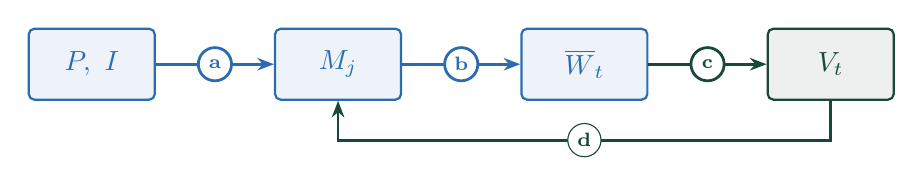
\begin{tikzpicture}[font=\normalsize,
  chainbox/.style={draw, rounded corners=2pt, line width=0.8pt, minimum width=1.6cm, minimum height=0.9cm},
  wat/.style={chainbox, draw=wfdy, fill=wfdy!8, text=wfdy},
  veg/.style={chainbox, draw=wfyr, fill=wfyr!8, text=wfyr},
  lk/.style={-{Stealth[length=6pt]}, line width=1pt},
  num/.style={circle, fill=white, draw, inner sep=0.5pt, font=\scriptsize\bfseries, minimum size=12pt}]
\definecolor{wfdy}{HTML}{2B6CB0}\definecolor{wfyr}{HTML}{18473C}
\node[wat] (a) {$P,\ I$};
\node[wat, right=1.5cm of a] (b) {$M_j$};
\node[wat, right=1.5cm of b] (c) {$\overline W_t$};
\node[veg, right=1.5cm of c] (d) {$V_t$};
\draw[lk, wfdy] (a) -- node[num, draw=wfdy, text=wfdy] {a} (b);
\draw[lk, wfdy] (b) -- node[num, draw=wfdy, text=wfdy] {b} (c);
\draw[lk, wfyr] (c) -- node[num, draw=wfyr, text=wfyr] {c} (d);
\draw[lk, wfyr] (d.south) -- ++(0,-0.5) -| (b.south);
\node[num, draw=wfyr, text=wfyr] at ($(c.south)+(0,-0.5)$) {d};
\end{tikzpicture}
\end{center}

\noindent \textcircled{\scriptsize a} Rain $P$ and irrigation $I$ fill a root-zone store $M_j$; \textcircled{\scriptsize b} the store decides the share $\overline W_t$ of the plants' water demand that is met; \textcircled{\scriptsize c} that share drives the change in cover $V_t$ through growth against decay and wind damage; \textcircled{\scriptsize d} cover in turn sets next year's demand on the store and how much wind reaches the ground, closing the loop. 

Figure~\ref{fig:m1-struct} adds the data behind each link. The reference section is the Yutian--Minfeng southern margin (Category~I in Section~\ref{sec:data}).

\begin{figure}[!htb]
  \centering
  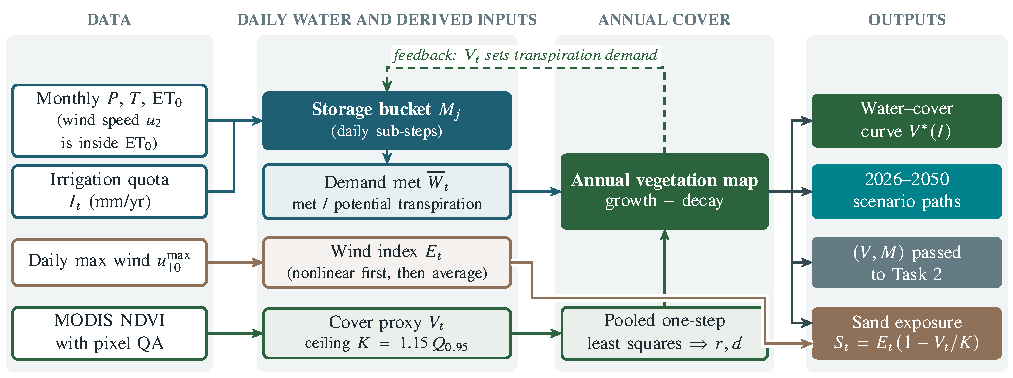
\includegraphics[width=\linewidth]{m1_structure.pdf}
  \caption{Structure of Model 1. }
  \label{fig:m1-struct}
\end{figure}

\subsection{Model construction}
\paragraph{Two states on two clocks.} The model tracks two quantities, and each one changes at its own natural speed. We picture them as two nested clocks (Figure~\ref{fig:m1-clocks}).
\begin{itemize}
  \item \textbf{Year clock (outer, slow) --- cover $V_t$ (\%).} It ticks \textbf{once per year}. Plants gain or lose cover over a season, and the satellite cover proxy is a single growing-season value, so a yearly step matches both biology and data.
  \item \textbf{Day clock (inner, fast) --- plant-available water $M_j$ (mm).} It ticks \textbf{365 times per year}. Rain and irrigation arrive in pulses and are used up within days; a yearly average would smooth away exactly the dry spells that stress plants.
\end{itemize}
\noindent The two clocks talk to each other at two points only, both at the year boundary:
\begin{itemize}
  \item \textbf{\textcircled{\scriptsize 1} Down (year $\to$ day).} At the start of each year, cover $V_t$ is \textbf{frozen} and sets each day's water demand $D_j$: a denser stand wants more water.
  \item \textbf{\textcircled{\scriptsize 2} Up (day $\to$ year).} At the end of each year, the 365 daily results are condensed into \textbf{one number}, the water-satisfaction ratio $\overline W_t$, which moves the outer ring from $V_t$ to $V_{t+1}$.
\end{itemize}
\noindent The water store $M$ is not reset: the last day of one year is the first day of the next, so wet or dry years carry over.

\begin{figure}[!htb]
  \centering
  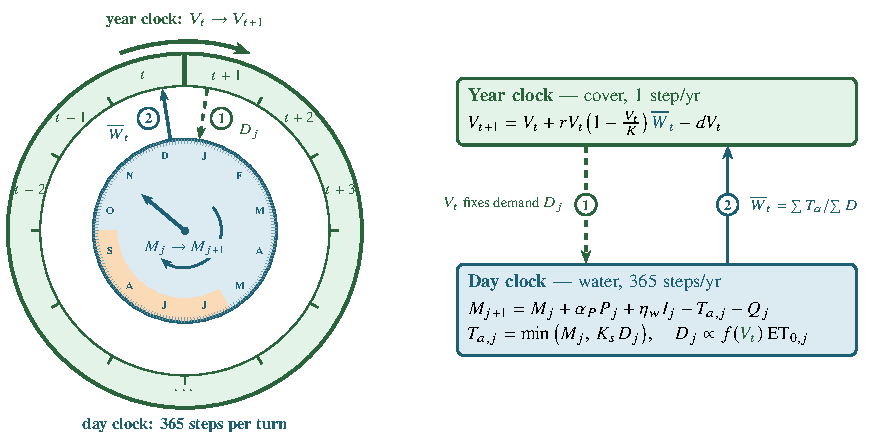
\includegraphics[width=\linewidth]{m1_two_clocks.pdf}
  \caption{The two clocks of Model 1 and their handoffs \textcircled{\scriptsize 1} and \textcircled{\scriptsize 2}.}
  \label{fig:m1-clocks}
\end{figure}

\paragraph{Cover equation: growth, decay, wind.}
\begin{equation}\label{eq:m1-veg}
V_{t+1}=V_t+\underbrace{rV_t\Big(1-\frac{V_t}{K}\Big)\overline W_t}_{\text{growth, limited by water}}
-\underbrace{dV_t}_{\text{natural decay}}
-\underbrace{kE_t\Big(1-\eta\frac{V_t}{K}\Big)V_t}_{\text{wind damage, reduced by shelter}}
\end{equation}
\emph{Growth} is logistic, stops at the local ceiling $K$, and is scaled by the water-satisfaction ratio $\overline W_t\in[0,1]$ (Eq.~\eqref{eq:m1-wbar}). \emph{Decay} removes a fixed share $d$ of cover each year. \emph{Wind damage} rises with the wind index $E_t$ (Section~\ref{sec:data}) and is reduced by the shelter factor $(1-\eta V_t/K)$ as cover thickens. Since $V=0$ stays at $0$, every scenario starts from a planted cover.

\paragraph{Water store: a daily bucket.} The root zone is treated as a bucket of capacity $C$ (Figure~\ref{fig:m1-bucket}). On each day $j$,
\begin{equation}\label{eq:m1-bucket}
\underbrace{M_{j+1}}_{\text{store tomorrow}}=\underbrace{M_j}_{\text{store today}}+\underbrace{\alpha_PP_j+\eta_wI_j}_{\text{effective inflow}}-\underbrace{T_{a,j}}_{\text{transpiration}}-\underbrace{Q_j}_{\text{overflow}},
\qquad T_{a,j}=\min\big(M,\ K_s(M)\,D_j\big).
\end{equation}
Only shares $\alpha_P$ of rain and $\eta_w$ of irrigation reach the roots, and water above capacity is lost ($Q_j$). The daily demand and the stress coefficient are
\begin{equation}\label{eq:m1-demand}
D_j=c\,\min\!\Big(1,\frac{2V_t}{V_{\mathrm{full}}}\Big)\,f(T_j)\,\mathrm{ET}_{0,j},\qquad
K_s=\min\Big\{1,\ \frac{M_j}{(1-p)C}\Big\}.
\end{equation}
The transpiration coefficient $c$ scales reference evapotranspiration $\mathrm{ET}_0$ to the demand of a full stand. Demand grows with cover until $V_t$ reaches half of the full-cover value $V_{\mathrm{full}}$, which is where cover feeds back on water, and $f(T)=\min\{1,\max\{0,(T-5)/20\}\}$ switches it on with the season. Below the stress threshold $(1-p)C$, the FAO-56 coefficient $K_s$ \cite{REF11} cuts transpiration in proportion to what is left (Figure~\ref{fig:m1-bucket}). Each daily step conserves water exactly.

\begin{figure}[!htb]
  \centering
  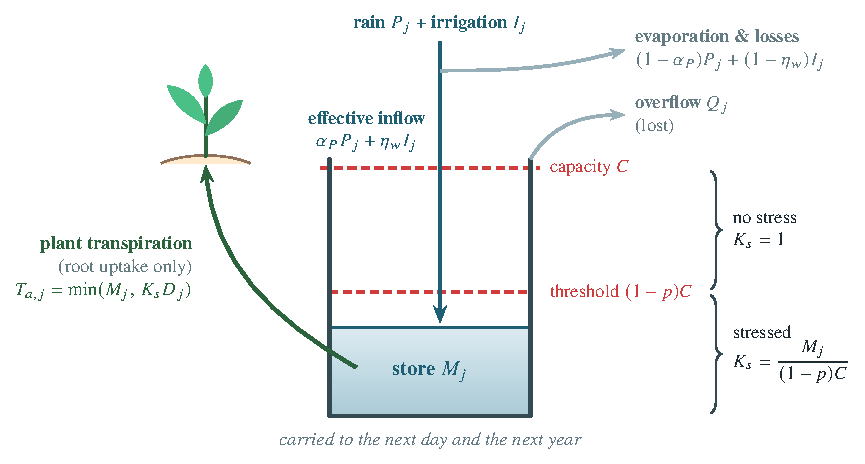
\includegraphics[width=0.95\linewidth]{m1_bucket.pdf}
  \caption{One daily step of the water bucket. $K_s$ threshold comes from reference FAO-56\cite{REF11} }
  \label{fig:m1-bucket}
\end{figure}

\paragraph{The link between the two clocks.} The daily bucket and the yearly cover update are coupled through one number, the water-satisfaction ratio
\begin{equation}\label{eq:m1-wbar}
\overline W_t=\frac{\sum_{j\in t}T_{a,j}}{\sum_{j\in t}D_j},
\end{equation}
the share of the plants' water demand actually met in year $t$. $\overline W_t=1$ means no water stress (as at the oases) and full growth rate $r$; $\overline W_t=0.4$ cuts growth to $0.4\,r$; $\overline W_t=0$ stops growth, leaving only decay and wind damage.

\subsection{Solution approach}
We fit growth and decay from data, step the coupled system through a year, and repeat the year to reach a long-run state or a scenario path.

\paragraph{Step 1: calibration by least squares.} At the seven oasis stations water is ample ($\overline W\approx1$) and wind damage is not separately identifiable, so we set $\overline W=1$ and $k=0$ there; growth and decay can then be estimated from cover alone. Fixing $K$ from each station's own record and writing $x=V/K$, Eq.~\eqref{eq:m1-veg} becomes
\begin{equation}\label{eq:m1-reg}
\underbrace{x_{s,t+1}-x_{s,t}}_{y_{s,t}:\ \text{observed change}}=r\,\underbrace{x_{s,t}(1-x_{s,t})}_{z_{1,s,t}:\ \text{growth signal}}-d\,\underbrace{x_{s,t}}_{z_{2,s,t}:\ \text{decay signal}}+\varepsilon_{s,t},
\end{equation}
where $s$ indexes stations and $\varepsilon_{s,t}$ is the one-step error. The model is linear in the unknowns $(r,d)$, so we estimate them by ordinary least squares over the set $\mathcal T$ of training pairs (target year $\le2022$, all seven stations pooled):
\begin{equation}\label{eq:m1-ls}
(\hat r,\hat d)=\arg\min_{r,d}\ \sum_{(s,t)\in\mathcal T}\big(y_{s,t}-r\,z_{1,s,t}+d\,z_{2,s,t}\big)^2 .
\end{equation}
Because the objective is quadratic in $(r,d)$, its minimiser has a closed form; Algorithm~\ref{alg:m1-ls} gives the procedure.

\begin{algorithm}[!htb]
\caption{Least-squares calibration of $r$ and $d$}\label{alg:m1-ls}
\begin{algorithmic}[1]
\Require training pairs $(x_{s,t},\,x_{s,t+1})$, $(s,t)\in\mathcal T$, with $N=|\mathcal T|$
\Ensure estimates $\hat r,\hat d$ and their bootstrap spread
\For{each pair $(s,t)\in\mathcal T$}
  \State $y_{s,t}\gets x_{s,t+1}-x_{s,t}$;\quad $z_{1,s,t}\gets x_{s,t}(1-x_{s,t})$;\quad $z_{2,s,t}\gets x_{s,t}$ \Comment{Eq.~\eqref{eq:m1-reg}}
\EndFor
\State Stack the pairs: $\bm y\in\mathbb R^{N}$ and design matrix $\bm Z=[\,\bm z_1,\ -\bm z_2\,]\in\mathbb R^{N\times2}$
\State Set the gradient of Eq.~\eqref{eq:m1-ls} to zero $\Rightarrow$ normal equations $\bm Z^\top\bm Z\,(\hat r,\hat d)^\top=\bm Z^\top\bm y$
\State Solve: $(\hat r,\hat d)^\top\gets\big(\bm Z^\top\bm Z\big)^{-1}\bm Z^\top\bm y$ \Comment{unique if columns of $\bm Z$ not proportional}
\For{$b=1,\dots,B$} \Comment{cluster bootstrap}
  \State Resample \emph{whole stations} with replacement; repeat lines 1--5 $\Rightarrow(\hat r^{(b)},\hat d^{(b)})$
\EndFor
\State Report $(\hat r,\hat d)$ with the spread of $\{(\hat r^{(b)},\hat d^{(b)})\}$
\State Check one-step error on hold-out pairs (2023--2025) against persistence $\hat x_{t+1}=x_t$
\end{algorithmic}
\end{algorithm}

\paragraph{Steps 2--3: one model year, then repeat.} Algorithm~\ref{alg:m1} shows the core loop. Repeating it under a typical climate year until $V$ and $M$ stop changing gives the long-run state for a given irrigation level. Because $\overline W$ depends on $V$, this fixed point is found numerically; we start from both a low and a high cover and accept the result only when both starts agree.

\begin{algorithm}[H]
\caption{One model year: the water store drives cover}\label{alg:m1}
\begin{algorithmic}[1]
\Require cover $V_t$, store $M$, irrigation $I_t$, one year of daily rain, ET$_0$ and temperature
\Ensure $V_{t+1}$, year-end store $M$, $\overline W_t$
\State Set daily demand $D_j$ from $V_t$ and the season \Comment{cover held fixed}
\For{each day $j$ of the year}
  \State $M\gets M+\alpha_PP_j+\eta_wI_j$;\quad spill anything above $C$ \Comment{inflow, overflow}
  \State $T_{a,j}\gets\min\big(M,K_s(M)D_j\big)$;\quad $M\gets M-T_{a,j}$ \Comment{stressed when $M$ is low}
\EndFor
\State $\overline W_t\gets\sum_jT_{a,j}/\sum_jD_j$ \Comment{Eq.~\eqref{eq:m1-wbar}}
\State $V_{t+1}\gets$ Eq.~\eqref{eq:m1-veg};\quad carry $M$ into next year
\end{algorithmic}
\end{algorithm}

\paragraph{Parameter values.} Table~\ref{tab:m1-par} lists the values used to solve the model. Only $r$ and $d$ are fitted; $K$ and $V_{\mathrm{full}}$ follow fixed rules applied to the data; the water and wind parameters cannot be fitted without field measurements, so they are stated assumptions with the ranges tested in the sensitivity analysis.

\begin{table}[H]
\centering\small
\renewcommand{\arraystretch}{1.1}
\begin{tabularx}{\linewidth}{@{}l X r c l@{}}
\toprule
Symbol & Meaning & Value & Range tested & Unit \\
\midrule
\multicolumn{5}{@{}l}{\textit{Fitted by least squares (Algorithm~\ref{alg:m1-ls})}}\\
$r$ & intrinsic growth rate & 0.547 & 0.335--1.168$^{\dagger}$ & yr$^{-1}$ \\
$d$ & natural decay rate & 0.107 & 0.077--0.202$^{\dagger}$ & yr$^{-1}$ \\
\midrule
\multicolumn{5}{@{}l}{\textit{Set from data by a fixed rule}}\\
$K$ & cover ceiling ($1.15\times$ 95th percentile of training cover) & 38.08 & -- & \% \\
$V_{\mathrm{full}}$ & cover at which demand is full (oasis end-member) & 66.59 & 64.85--69.40 & \% \\
\midrule
\multicolumn{5}{@{}l}{\textit{Assumed (no field data to fit)}}\\
$C$ & root-zone storage capacity & 75 & 30--150 & mm \\
$p$ & stress-free share of storage (FAO-56 \cite{REF11}) & 0.5 & 0.3--0.7 & -- \\
$c$ & transpiration coefficient & 1.0 & 0.7--1.2 & -- \\
$\eta_w$ & share of irrigation reaching the roots & 0.75 & 0.65--0.85 & -- \\
$\alpha_P$ & share of rain reaching the roots & 0.25 & 0--1 & -- \\
$k$ & wind-damage rate & 0 & 0--0.10 & -- \\
$\eta$ & shelter strength of dense cover & 1 & -- & -- \\
$u_T$ & wind threshold for sand drift & 5 & -- & m/s \\
$V_0$ & initial cover of a new stand & 2 & -- & \% \\
$M_0$ & initial store of a new stand & 37.5 & -- & mm \\
\bottomrule
\end{tabularx}
\caption{Model 1 parameters.}
\label{tab:m1-par}
\end{table}

\subsection{Results}
Results are for the Yutian--Minfeng section (127.95\,km $\times$ 1\,km) under a repeated 2015--2022 mean climate year; they compare water strategies, not forecasts of specific years.

\begin{figure}[!t]
  \centering
  \begin{subfigure}[t]{0.49\linewidth}
    \centering
    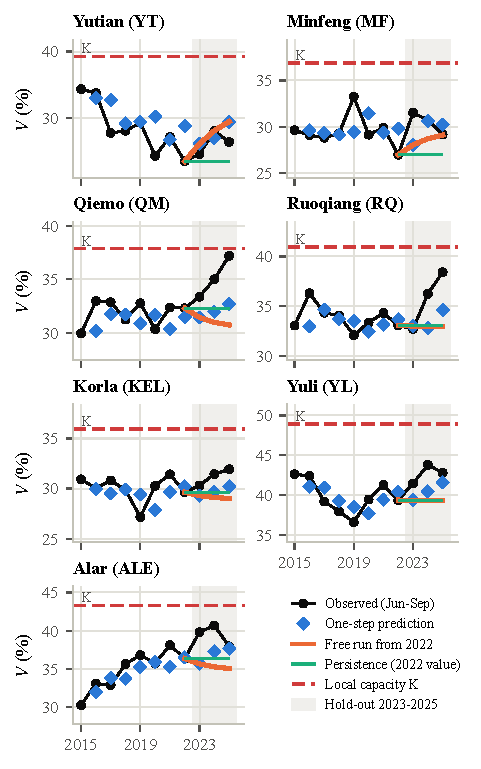
\includegraphics[width=\linewidth]{m1_f01_station_series_tall.pdf}
    \caption{Observed cover at the seven stations, 2015--2025.}
    \label{fig:m1-obs}
  \end{subfigure}\hfill
  \begin{subfigure}[t]{0.49\linewidth}
    \centering
    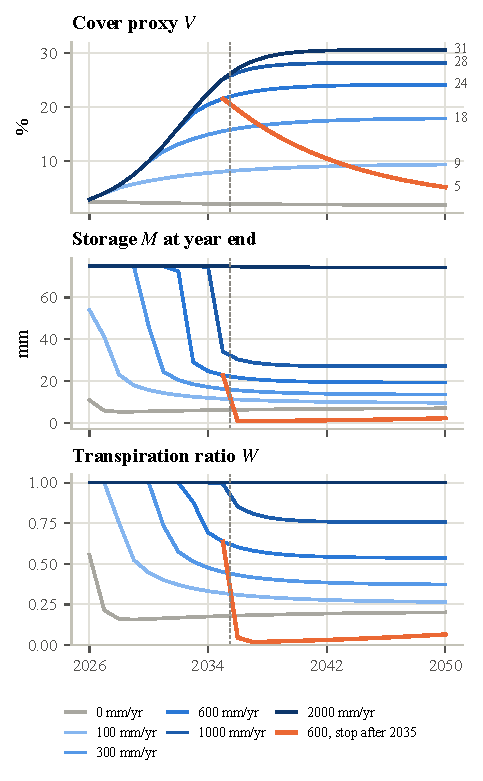
\includegraphics[width=\linewidth]{m1_f07_scenario_trajectories_tall.pdf}
    \caption{Scenario paths on the section, 2026--2050.}
    \label{fig:m1-scen}
  \end{subfigure}
  \caption{Cover and soil water over time: (a) observed, (b) modelled scenarios.}
  \label{fig:m1-paths}
\end{figure}

\paragraph{Model reliability.} An unwatered stand loses half its cover in about six years. On hold-out years the one-step forecast does not beat persistence overall (RMSE 0.064 vs 0.054 in $V/K$), but it does at Minfeng and Yutian, the two stations in our section. Figure~\ref{fig:m1-obs} shows why. Observed growing-season cover (black) varies between about 24\% and 44\% and stays below each station's ceiling $K$ (red dashed). The one-step predictions (blue) follow the level of each series but not its year-to-year spikes. In the hold-out years (grey band), cover rose sharply at Qiemo, Ruoqiang and Alar; the free run from 2022 (orange) stays near the 2022 value and misses this greening, for example 33.0\% against 38.4\% observed at Ruoqiang in 2025. At Yutian and Minfeng the free run follows the observed values more closely. Model~1 is therefore used to compare strategies, not to predict single years.
\newpage
\paragraph{Evolution of the state variables.} From a planted cover of 2\%, cover and soil water pass through three phases (Figure~\ref{fig:m1-scen}):
\begin{enumerate}\setlength{\itemsep}{1pt}\setlength{\parsep}{0pt}
  \item \textbf{Establishment: growth, not water, limits cover.} Young plants use little water, so with 300\,mm/yr or more the store stays full ($\overline W=1$) and the surplus drains. All such quotas give the same 9.9\% cover by 2030, so water above about 300\,mm/yr is wasted in this phase.
  \item \textbf{Transition: cover drains the store.} Demand rises with cover until it exceeds supply. The store then drops from capacity within about two years and settles slowly (to about 13\,mm at 300\,mm/yr), and $\overline W$ falls below one. This is the feedback at work: more cover means less water per plant, which slows growth.
  \item \textbf{Plateau (after 15--25 years): both settle.} Each quota gives its own steady cover and store, e.g.\ 17.9\% and 13\,mm at 300\,mm/yr, or 24.1\% and 19\,mm at 600\,mm/yr.
\end{enumerate}
The plateau lasts only while water is supplied. If irrigation stops after ten years, the store empties within a year, $\overline W$ falls to 0.03--0.07, and cover drops from 21.5\% to 12.7\% in five years and to 5.1\% in fifteen.

\paragraph{Controlling factors: water supply.} Water supply is the main control. Rain alone (52\,mm/yr against about 1,700\,mm/yr of evaporative demand) holds only 1.8\% cover.

\noindent\begin{minipage}[t]{0.585\linewidth}
\vspace{0pt}
Irrigation raises long-run cover quickly at first, then with strongly diminishing returns (Figure~\ref{fig:m1-curve}a):
\begin{enumerate}\setlength{\itemsep}{1pt}\setlength{\parsep}{0pt}
  \item the first 100\,mm/yr adds 7.7 percentage points;
  \item going from 500 to 600\,mm/yr adds only 1.6;
  \item above about 1,500\,mm/yr, cover stops at a ceiling of 30.6\%.
\end{enumerate}
The bucket explains this shape: at 300\,mm/yr only 37\% of demand is met (Figure~\ref{fig:m1-curve}b), so the deficit, not the ceiling $K$, keeps cover at 18\%; above 1,500\,mm/yr extra water only overflows.
\end{minipage}\hfill
\begin{minipage}[t]{0.395\linewidth}
\vspace{0pt}\centering
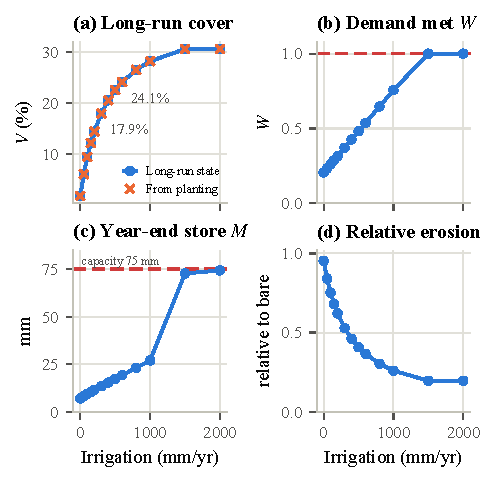
\includegraphics[width=\linewidth]{m1_f06_water_cover_curve_half.pdf}
\captionof{figure}{Long-run state against irrigation. Red dashed lines are limits.}
\label{fig:m1-curve}
\end{minipage}

\noindent\begin{minipage}[t]{0.615\linewidth}
\vspace{0pt}
\paragraph{Controlling factors: demand, delivery and wind.} With water supply fixed, we varied the other factors one at a time (Figure~\ref{fig:m1-sens}). They fall into three groups:
\begin{enumerate}\setlength{\itemsep}{1pt}\setlength{\parsep}{0pt}
  \item \textbf{Factors that shift long-run cover by 1--3 points:} the transpiration coefficient $c$ ($-1.7$ to $+3.4$ points at 300\,mm/yr), irrigation efficiency ($\pm1.2$) and the effective rain fraction ($-0.5$ to $+1.4$). All three act through $\overline W$, the supply-to-demand ratio.
  \item \textbf{Factors that change soil water but not long-run cover:} storage capacity and the stress threshold. Without overflow, all inflow is eventually transpired, so $\overline W$ depends only on inflow and demand; these factors change only the storage level and its timing.
  \item \textbf{Wind damage, the largest uncertainty.} The data cannot pin down its rate, so it is a scenario; at the highest rate tested it cuts cover at 300\,mm/yr by 24\% (17.9\% to 13.6\%), more than any water parameter.
\end{enumerate}

\paragraph{Summary.} Cover and soil water rise together, settle at a level set by the water supply, and decline once water stops. Water supply is the main control, with sharply diminishing returns; demand, delivery efficiency and wind damage shift the result.
\end{minipage}\hfill
\begin{minipage}[t]{0.365\linewidth}
\vspace{0pt}\centering
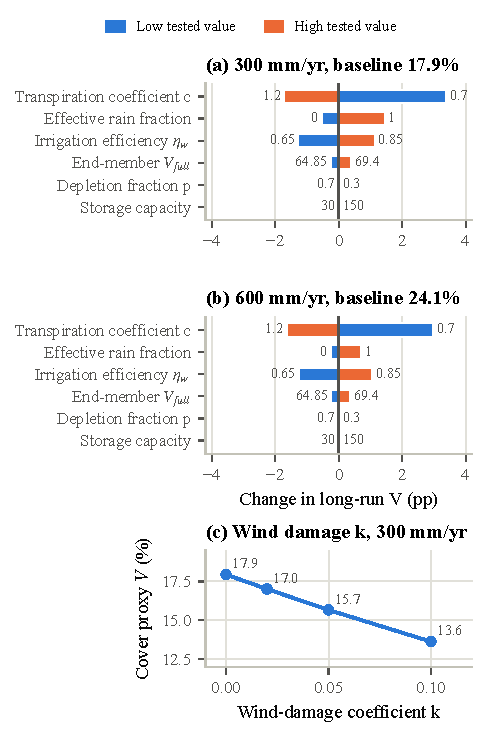
\includegraphics[width=\linewidth]{m1_f09_sensitivity_tall.pdf}
\captionof{figure}{Sensitivity of long-run cover to one-at-a-time changes and to wind damage.}
\label{fig:m1-sens}
\end{minipage}

% Model 2 sketch: concise logic chain, 4 core formulas, visual restriction chart,
% and results aligned with Task 2's three questions in Problem B.
\clearpage
\section{Model 2: Optimal Investment, Scheduling and Resource Allocation}\label{sec:model2}
Task~2 turns Model~1 into a 15-year dynamic decision problem: how much belt to plant each year, how to schedule ecological water and labour, and how to split funds among construction, O\&M and photovoltaics (PV) under a fixed budget:

\begin{center}
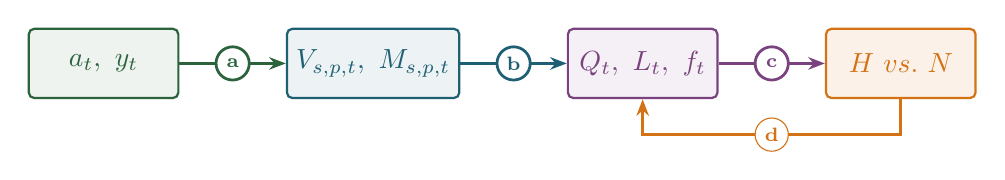
\begin{tikzpicture}[font=\normalsize,
  chainbox/.style={draw, rounded corners=2pt, line width=0.8pt, minimum width=1.9cm, minimum height=0.88cm, align=center},
  dec/.style={chainbox, draw=wfyr, fill=wfyr!8, text=wfyr},
  wat/.style={chainbox, draw=wfdy, fill=wfdy!8, text=wfdy},
  fin/.style={chainbox, draw=wfpl, fill=wfpl!8, text=wfpl},
  pvc/.style={chainbox, draw=wfpv, fill=wfpv!10, text=wfpv},
  lk/.style={-{Stealth[length=6pt]}, line width=1pt},
  num/.style={circle, fill=white, draw, inner sep=0.5pt, font=\scriptsize\bfseries, minimum size=12pt}]
\definecolor{wfdy}{HTML}{1E5F74}\definecolor{wfyr}{HTML}{2B633C}\definecolor{wfpl}{HTML}{7A437F}\definecolor{wfpv}{HTML}{D47216}
\node[dec] (a) {$a_t,\ y_t$};
\node[wat, right=1.35cm of a] (b) {$V_{s,p,t},\ M_{s,p,t}$};
\node[fin, right=1.35cm of b] (c) {$Q_t,\ L_t,\ f_t$};
\node[pvc, right=1.35cm of c] (d) {$H\ \text{vs.}\ N$};
\draw[lk, wfyr] (a) -- node[num, draw=wfyr, text=wfyr] {a} (b);
\draw[lk, wfdy] (b) -- node[num, draw=wfdy, text=wfdy] {b} (c);
\draw[lk, wfpl] (c) -- node[num, draw=wfpl, text=wfpl] {c} (d);
\draw[lk, wfpv] (d.south) -- ++(0,-0.45) -| (c.south);
\node[num, draw=wfpv, text=wfpv] at ($(c.south)!0.5!(d.south)+(0,-0.45)$) {d};
\end{tikzpicture}
\end{center}

\noindent \textcircled{\scriptsize a} Annual planting $a_t$ and PV builds $y_t$ create dated cohorts; \textcircled{\scriptsize b} each cohort carries its own Model~1 cover and soil-water state $(V,M)$; \textcircled{\scriptsize c} all active stocks demand water $Q_t$, labour $L_t$ and spending shares $f_t=(f_t^b,f_t^o,f_t^p)$; \textcircled{\scriptsize d} PV income lowers discounted net cost $N$ while competing with belt expansion for upfront budget, framing an explicit trade-off against ecological benefit $H$ (Figure~\ref{fig:m2-struct}).

\begin{figure}[!htb]
  \centering
  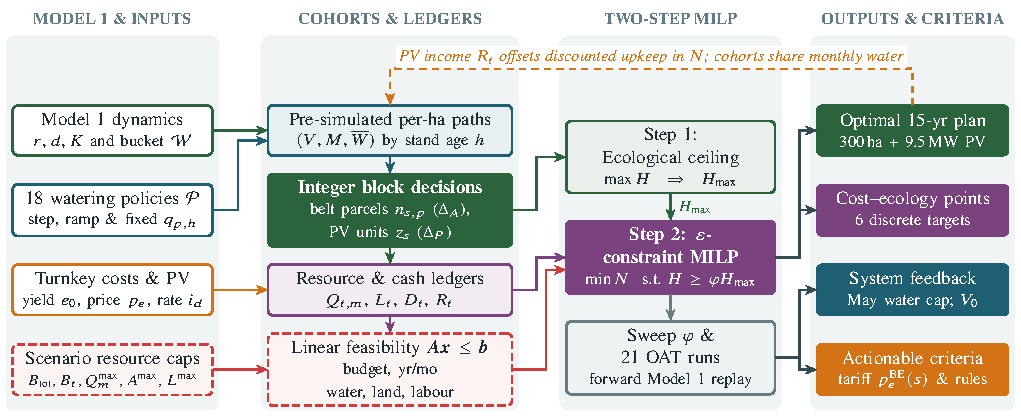
\includegraphics[width=\linewidth]{m2_structure.pdf}
  \caption{Structure of Model~2. Pre-simulated Model~1 cohort paths make all ledgers linear in block decisions.}
  \label{fig:m2-struct}
\end{figure}

\subsection{Model construction}
\paragraph{Cohort idea and ecological benefit.} Tracking only total area $A_t$ cannot distinguish a newly planted shrub ($V_0=2\%$, low water demand) from an older stand ($>12\%$ cover, high summer demand). Instead, we define a \textbf{cohort} $(s,p)$ by its planting year $s\in\{1,\dots,T\}$ and lifetime watering schedule $p\in\mathcal P$ ($18$ schedules: constant $0\text{--}1{,}000$\,mm/yr, step-up or step-down after age $3$ or $5$, and a $100\to300\to600$\,mm/yr ramp). Belt land is chosen in integer blocks $a_{s,p}=\Delta_A n_{s,p}$ ($\Delta_A=50$\,ha) and PV in blocks $y_s=\Delta_P z_s$ ($\Delta_P=100$\,kW), giving active belt stock $A_t=\sum_{s\le t,p}a_{s,p}$, installed PV $P_t^{\mathrm{inst}}=\sum_{s\le t}y_s$, and operating PV $P_t^{\mathrm{op}}=\sum_{s<t}y_s$ (panels built in year $s$ generate from year $s+1$).

Each cohort runs Model~1's daily water bucket $\mathcal W$ (Algorithm~\ref{alg:m1}) under its age-specific quota $q_{p,t-s}$ and updates cover via Eq.~\eqref{eq:m1-veg}. Summing start-of-year cover relative to the local ceiling $K$ across all active cohorts defines the 15-year ecological benefit:
\begin{equation}\label{eq:m2-eco}
H=\sum_{t=1}^{T}\sum_{s\le t,\,p\in\mathcal P}\underbrace{a_{s,p}\,\frac{V_{s,p,t}}{K}}_{\text{effective ha in year }t},\qquad
(M_{s,p,t+1},\,\overline W_{s,p,t})=\mathcal W\!\big(V_{s,p,t},\,M_{s,p,t},\,q_{p,t-s}\big).
\end{equation}
One hectare at $V=K$ for one year scores $1\text{ effective ha}\cdot\text{yr}$. Using start-of-year cover $V_{s,p,t}$ avoids crediting growth before it happens and naturally rewards early planting because desert shrubs take a decade to mature. Because separate strips do not share soil water, running Model~1 \emph{once per schedule} beforehand fixes $V_{s,p,t}$ per hectare, making $H$ strictly linear in $n_{s,p}$.

\paragraph{Investment allocation ratios and PV revenue.} In year $t$, gross spending $D_t$ splits across Task~2's three required uses---construction, O\&M (including water delivery $Q_t$), and PV capital---while operating panels earn electricity revenue $R_t$:
\begin{equation}\label{eq:m2-cash}
D_t=\underbrace{c_b a_t}_{C_t^b:\ \text{build}}+\underbrace{\big(c_m A_t+c_{pm}P_t^{\mathrm{op}}+c_w Q_t\big)}_{C_t^o:\ \text{O\&M + water}}+\underbrace{c_p y_t}_{C_t^p:\ \text{PV}},\quad
R_t=p_e\!\sum_{s<t}y_s e_0(1-d_p)^{t-s-1}.
\end{equation}
Here $a_t=\sum_p a_{t,p}$ is newly treated area, $(f_t^b,f_t^o,f_t^p)=(C_t^b,C_t^o,C_t^p)/D_t$ ($f_t^b+f_t^o+f_t^p=1$ when $D_t>0$) is the annual \textbf{investment allocation ratio}, $e_0$ is first-year net grid yield per kW, $d_p=0.5\%/\text{yr}$ is panel degradation \cite{EN06}, and $p_e$ is the settlement tariff \cite{CN06,EN05}.

\paragraph{System restrictions and explicit trade-off.} Rather than listing separate constraint equations, Figure~\ref{fig:m2-caps} maps how all four resource dimensions---funding, water, land/grid and labour---constrain both new construction flows and cumulative stocks in service. Capital is paid at the start of year $t$ and O\&M/revenue occur at year-end (real discount factor $\delta=(1+i_d)^{-1}$). Instead of inventing a subjective money price for vegetation, we formulate the ecology--cost trade-off via a two-step $\varepsilon$-constraint problem:
\begin{equation}\label{eq:m2-eps}
\min_{\bm n,\bm z}\ N=\sum_{t=1}^{T}\Big[\underbrace{\delta^{t-1}\big(C_t^b+C_t^p\big)}_{\text{year-start capex}}+\underbrace{\delta^{t}\big(C_t^o-R_t\big)}_{\text{year-end O\&M $-$ PV}}\Big]
\;\;\text{s.t.}\;\; H\ge\varphi H_{\max},\ \text{caps in Fig.~\ref{fig:m2-caps}},
\end{equation}
where Step~1 maximises $H$ under the same caps to find the physical ceiling $H_{\max}$, and Step~2 minimises net present cost $N$ for a chosen ecological target share $\varphi\in[0,1]$ ($\varphi=0.60$ in the baseline).

\begin{figure}[!htb]
  \centering
  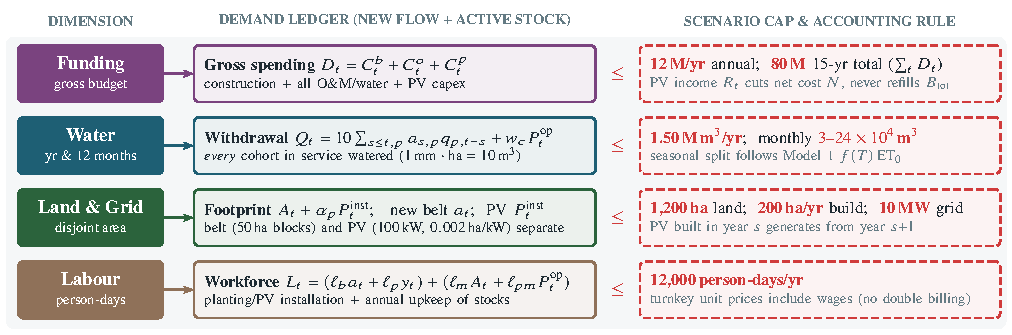
\includegraphics[width=\linewidth]{m2_restrictions.pdf}
  \caption{Resource restrictions and accounting rules of Model~2 across funding, water, land/grid and labour.}
  \label{fig:m2-caps}
\end{figure}

\subsection{Solution approach}
Pre-simulating the 18 schedules in Model~1 converts Eq.~\eqref{eq:m2-eps} into an exact mixed-integer linear programme (MILP) over integer block counts $\bm x=(\bm n,\bm z)$, solved via branch-and-cut (HiGHS, MIP gap tolerance $0.20\%$; Algorithm~\ref{alg:m2-milp}). Every solved plan is independently replayed forward through Model~1 to verify water and cash closure (maximum discrepancy $1.9\times10^{-9}$). Because the problem statement gives no site budget, water quota or tariff, Table~\ref{tab:m2-par} sets an auditable 15-year planning scenario anchored to a 2024 Yutian desert-treatment trial ($52{,}500$\,CNY/ha \cite{REF20}) and literature PV degradation \cite{EN06}.

\begin{algorithm}[!htb]
\caption{Cohort pre-simulation and two-step $\varepsilon$-constraint MILP}\label{alg:m2-milp}
\begin{algorithmic}[1]
\Require Model~1 $(r,d,K,\mathcal W)$, 18-policy library $\mathcal P$, scenario parameters and caps (Table~\ref{tab:m2-par}, Figure~\ref{fig:m2-caps})
\Ensure optimal schedule $\bm x^*$, ceiling $H_{\max}$, trade-off points and sensitivity runs
\State Run Model~1 (Algorithm~\ref{alg:m1}) once per policy $p\in\mathcal P$ from $(V_0,M_0)$ to tabulate per-ha $V_{\mathrm{start}}$ and monthly water
\State Build linear constraint matrix $\bm A\bm x\le\bm b$, ecology vector $\bm h$ (Eq.~\eqref{eq:m2-eco}) and net cost vector $\bm c$ (Eq.~\eqref{eq:m2-eps})
\State \textbf{Step 1:} $H_{\max}\gets\max\{\bm h^\top\bm x:\bm A\bm x\le\bm b,\ \bm x\in\mathbb Z_{\ge0}^m\}$;\quad \textbf{Step 2:} $\bm x^*\gets\arg\min\{\bm c^\top\bm x:\bm A\bm x\le\bm b,\ \bm h^\top\bm x\ge\varphi H_{\max}\}$
\State Sweep $\varphi\in\{0,0.2,\dots,1.0\}$; perturb parameters at fixed $H\ge0.60\,H_{\max}$; replay chosen cohorts in Model~1
\end{algorithmic}
\end{algorithm}

\begin{table}[!htb]
\centering\small
\renewcommand{\arraystretch}{1.06}
\begin{tabularx}{\linewidth}{@{}l X r c l@{}}
\toprule
Symbol & Meaning & Base value & Tested / note & Unit \\
\midrule
$T;\ \Delta_A,\Delta_P$ & horizon; belt block and PV block ($V_0=2\%$, $M_0=37.5$\,mm) & $15;\ 50,\ 100$ & $V_0$: 1--4\% & yr; ha, kW \\
$c_b,\ c_m,\ c_w$ & planting capex \cite{REF20}, belt O\&M, water unit cost & $52{,}500,\ 1{,}500,\ 1.0$ & $c_b\pm25\%$, $c_m\pm50\%$ & CNY (ha, m$^3$) \\
$c_p,\ c_{pm}$ & PV turnkey capex and annual O\&M rate & $3{,}000,\ 50$ & $c_p\pm25\%$ & CNY/kW \\
$e_0,\ p_e,\ d_p$ & 1st-yr PV yield, tariff, degradation \cite{EN06} ($w_c=0.02$\,m$^3$/kW) & $1{,}500,\ 0.30,\ 0.5\%$ & $p_e$: 0.15--0.40 & kWh, CNY, /yr \\
$\ell_b,\ell_m;\ \ell_p,\ell_{pm}$ & belt build/O\&M and PV build/O\&M labour rates & $30,3;\ 0.10,0.01$ & turnkey wages & p-d / (ha, kW) \\
$i_d;\ \varphi$ & real discount rate; baseline ecological target share & $5\%;\ 60\%$ & $\varphi$: 0--100\% & -- \\
\bottomrule
\end{tabularx}
\caption{Key Model~2 scenario parameters (caps shown in Figure~\ref{fig:m2-caps}; Model~1 inputs in Table~\ref{tab:m1-par}).}
\label{tab:m2-par}
\end{table}

\subsection{Results}
\paragraph{Optimal 15-year trajectory and ecology--cost trade-off.} Putting all resources into vegetation gives $H_{\max}=2{,}097.0\text{ effective ha}\cdot\text{yr}$ ($900$\,ha planted, $0$\,MW PV, $N=64.42$\,M\,CNY). At the $\varphi=60\%$ target ($1{,}258.2\text{ effective ha}\cdot\text{yr}$), the optimal schedule (Figure~\ref{fig:m2-plan}) plants $300$\,ha in years 1--2 ($150$\,ha/yr: $250$\,ha on $100\to300$\,mm/yr after age~3, $50$\,ha on $100\to300\to600$\,mm/yr) and installs $9.5$\,MW of PV across years 1--4 ($1.2,1.1,3.7,3.5$\,MW), reaching $H=1{,}264.8\text{ effective ha}\cdot\text{yr}$ at net present cost $N=25.35$\,M\,CNY (MIP gap $0.20\%$).

Three mechanisms shape the four decision trajectories in Figure~\ref{fig:m2-plan}. First, \textbf{front-loading}: years 1--4 use virtually the entire $12$\,M/yr cap, shifting allocation ratios from $66\%$ planting / $30\%$ PV in year~1 to $\sim90\%$ PV in years 3--4 and $100\%$ O\&M thereafter; from year~5, PV revenue ($4.05\text{--}4.25$\,M/yr) covers more than twice annual O\&M and water ($1.83\text{--}1.98$\,M/yr), saving $2.49$\,M ($9.0\%$) over the best no-PV plan ($27.84$\,M). Second, \textbf{age-stepped watering}: giving young seedlings $100$\,mm/yr in ages 1--3 avoids overflowing Model~1's root bucket ($6.6\%$ cheaper than constant quotas), before stepping up as canopy demand grows. Third, \textbf{seasonal bottleneck}: annual water peaks at $1.05\text{ M m}^3\text{/yr}$ ($70\%$ of the annual cap) and labour at $5{,}522$\,p-d ($46\%$), yet \textbf{May water use hits $95\%$ of the monthly cap} in years 8--15---showing that spring delivery, not annual volume, is the true physical constraint.

\begin{figure}[!htb]
  \centering
  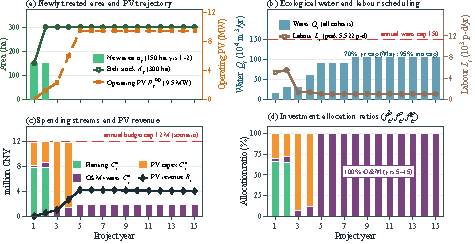
\includegraphics[width=\linewidth]{m2_plan.pdf}
  \caption{Optimal 15-year trajectories of Task~2's four decision groups ($\varphi=60\%$ scenario): (a) newly treated area and operating PV, (b) ecological water and labour scheduling, (c) spending streams vs.\ PV revenue, (d) annual investment allocation ratios.}
  \label{fig:m2-plan}
\end{figure}

Sweeping $\varphi$ from $0\%$ to $100\%$ across six separate MILP solves reveals a sharp cost bend (Figure~\ref{fig:m2-tradeoff}). Up to $\varphi=60\%$, each extra effective $\text{ha}\cdot\text{yr}$ costs $22.6\text{--}26.3$\,k\,CNY while PV stays at $9.5\text{--}10$\,MW. Above $60\%$, marginal cost more than doubles to $36.7$\,k ($80\%$) and $57.1$\,k\,CNY ($100\%$) because higher cover pushes stands into Model~1's diminishing-returns regime and crowds PV out of the $80$\,M gross budget ($10\to5.3\to0$\,MW).

\begin{figure}[!htb]
  \centering
  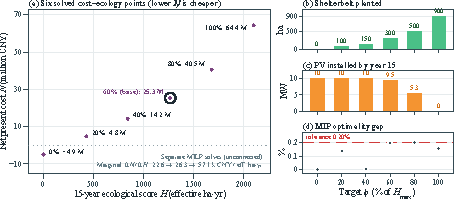
\includegraphics[width=\linewidth]{m2_tradeoff.pdf}
  \caption{Explicit ecology--cost trade-off across six discrete MILP solves (unconnected scenario points; MIP gap $\le0.20\%$).}
  \label{fig:m2-tradeoff}
\end{figure}

\paragraph{Sensitivity of the investment structure.} Holding the ecological requirement fixed at $H\ge1{,}258.2\text{ effective ha}\cdot\text{yr}$ isolates how prices, O\&M and physical assumptions reshape the investment mix (Figure~\ref{fig:m2-sensitivity}):
\begin{enumerate}\setlength{\itemsep}{1pt}\setlength{\parsep}{0pt}
  \item \textbf{PV is all-or-nothing on tariff and capex.} At $0.15$\,CNY/kWh or $3{,}750$\,CNY/kW capex, optimal PV drops to $0$\,MW ($N=27.8$\,M, $+9.8\%$); at $0.40$\,CNY/kWh or $2{,}250$/kW capex, PV hits the $10$\,MW cap and cuts net cost by $30\text{--}44\%$. Forcing PV share $\ge30\%$ has zero effect in the baseline ($41.3\%$ PV share already), showing PV should follow price rather than a fixed quota.
  \item \textbf{O\&M and planting costs shift PV headroom.} Raising O\&M unit rates by $+50\%$ increases $N$ by $+14.8\%$ and squeezes PV down to $5.6$\,MW to preserve maintenance funds; $\pm25\%$ planting capex shifts $N$ by $\pm18\%$.
  \item \textbf{Initial survival $V_0$ outweighs secondary parameters.} Dropping initial cover from $2\%$ to $1\%$ forces $400$\,ha of planting and raises cost $+29.1\%$ ($32.7$\,M), whereas $V_0=4\%$ needs $200$\,ha ($-19.5\%$). Cutting water caps by $20\%$ raises cost $+9.7\%$ ($350$\,ha), while halving labour or refining blocks to $25$\,ha ($-0.22\%$) lies within solver tolerance.
\end{enumerate}

\begin{figure}[!htb]
  \centering
  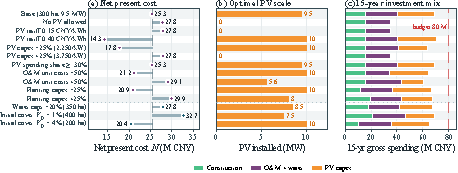
\includegraphics[width=0.95\linewidth]{m2_sensitivity.pdf}
  \caption{Sensitivity of net cost, PV scale and 15-year investment structure at fixed ecological target ($1{,}258.2\text{ effective ha}\cdot\text{yr}$).}
  \label{fig:m2-sensitivity}
\end{figure}

\paragraph{Actionable process criterion.} A standalone $1$\,kW PV unit built in year $s<T$ pays back its capex, O\&M and washing water within the horizon if and only if the tariff exceeds the break-even threshold
\begin{equation}\label{eq:m2-be}
p_e\ge p_e^{\mathrm{BE}}(s)=\frac{c_p+\sum_{t=s+1}^{T}\delta^{t-s+1}\,(c_{pm}+c_w w_c)}{\sum_{t=s+1}^{T}\delta^{t-s+1}\,e_0(1-d_p)^{t-s-1}}.
\end{equation}
\noindent\begin{minipage}[t]{0.54\linewidth}
\vspace{0pt}
In the baseline, $p_e^{\mathrm{BE}}(s)$ rises from $0.253$\,CNY/kWh in year~1 to $0.293$ in year~4 and crosses $0.30$ in year~5 ($0.312$, Figure~\ref{fig:m2-pv}a), matching the MILP's exact build window (years 1--4). This gives four field rules:
\begin{enumerate}\setlength{\topsep}{2pt}\setlength{\itemsep}{0pt}\setlength{\parsep}{0pt}
  \item \textbf{Two-gate PV rule:} install PV in year $s$ only if $p_e\ge p_e^{\mathrm{BE}}(s)$ \emph{and} budget slack remains after planting.
  \item \textbf{Plant in years 1--2:} front-load belt construction so shrubs accrue cover across the full horizon.
  \item \textbf{Ramp water by stand age:} supply $100$\,mm/yr in ages 1--3, step to $300$\,mm/yr at age~4, and $600$\,mm/yr (age $8+$) on core strips.
  \item \textbf{Size for May \& audit $V_0$:} dispatch against May--July water caps, secure $V_0\ge2\%$ via pilot plots, and target the $40\text{--}60\%$ cost knee.
\end{enumerate}
\end{minipage}\hfill
\begin{minipage}[t]{0.43\linewidth}
\vspace{0pt}\raggedleft
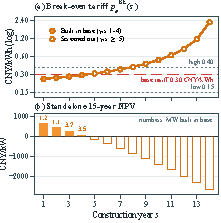
\includegraphics[width=0.90\linewidth]{m2_pv_screen.pdf}
\captionof{figure}{Standalone PV entry screen by build year $s$ (excludes resource opportunity cost).}
\label{fig:m2-pv}
\end{minipage}

\paragraph{Summary.} Cohort pre-simulation embeds Model~1's water--cover physics into a linear multi-year allocation model. Front-loading belt planting in years 1--2, stepping water up with stand age, and building PV only while $p_e\ge p_e^{\mathrm{BE}}(s)$ cuts net cost by $9\%$ and funds long-term upkeep, while identifying May water delivery and seedling survival $V_0$ as the critical vulnerabilities tested under stochastic disasters in Model~3.

% Model 3: concise logic chain, 3 core equations, visual Discreteness & Matrix chart,
% and stress-test results aligned with Task 3 of CQU Problem B (no M1 sensitivity overlap).
\clearpage
\section{Model 3: Post-Construction Resilience under Compound Disasters}\label{sec:model3}
Task~3 asks whether the belt planned in Model~2 can withstand disasters and recover. Starting from Model~2's year~15 ($t=0$), we follow the belt for 50 more years through four links:

\begin{center}

\begin{tikzpicture}[font=\normalsize,
  chainbox/.style={draw, rounded corners=2pt, line width=0.8pt, minimum width=1.95cm, minimum height=0.88cm, align=center},
  haz/.style={chainbox, draw=pSand, fill=pSand!10, text=pSand},
  wat/.style={chainbox, draw=pWater, fill=pWater!8, text=pWater},
  veg/.style={chainbox, draw=pVeg, fill=pVeg!8, text=pVeg},
  cen/.style={chainbox, draw=pPlum, fill=pPlum!8, text=pPlum},
  lk/.style={-{Stealth[length=6pt]}, line width=1pt},
  num/.style={circle, fill=white, draw, inner sep=0.5pt, font=\scriptsize\bfseries, minimum size=12pt}]
\node[haz] (a) {$D_t^{\mathrm{dr}},\ R_t$};
\node[wat, right=1.30cm of a] (b) {$I_{j,t,m}\xrightarrow{\Phi}\widetilde V$};
\node[veg, right=1.30cm of b] (c) {$V_{j,t+1},\ M_{j,t+1}$};
\node[cen, right=1.30cm of c] (d) {$\tau_{\mathrm{proj}}\ \text{vs.}\ H_{\mathrm{eco}}$};
\draw[lk, pSand]  (a) -- node[num, draw=pSand, text=pSand] {a} (b);
\draw[lk, pWater] (b) -- node[num, draw=pWater, text=pWater] {b} (c);
\draw[lk, pPlum]  (c) -- node[num, draw=pPlum, text=pPlum] {c} (d);
\draw[lk, pVeg]   (c.south) -- ++(0,-0.45) -| (b.south);
\node[num, draw=pVeg, text=pVeg] at ($(b.south)!0.5!(c.south)+(0,-0.45)$) {d};
\end{tikzpicture}
\end{center}

\noindent \textcircled{\scriptsize a} Droughts and storms arrive at random; \textcircled{\scriptsize b} rationed canal water drives Model~1's water--cover map $\Phi$; \textcircled{\scriptsize c} each year we check whether half the belt is below the warning level; \textcircled{\scriptsize d} the stands keep growing afterwards, so they can \textbf{recover} (Figure~\ref{fig:m3-struct}).

\begin{figure}[!htb]
  \centering
  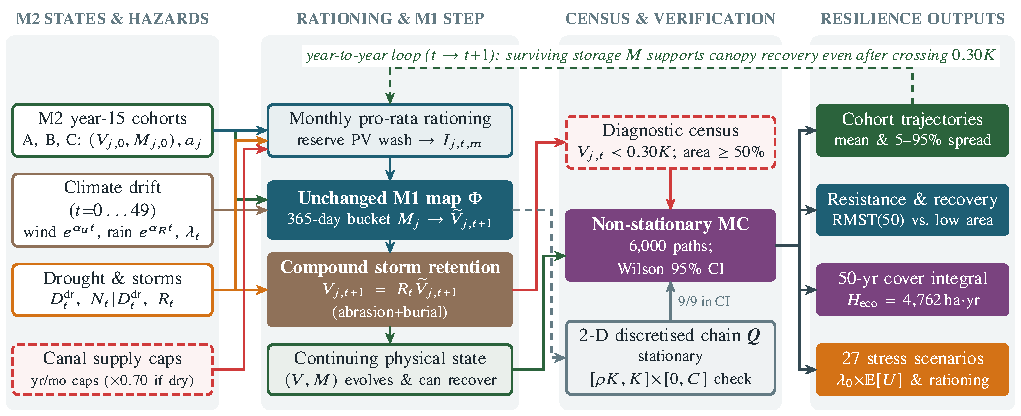
\includegraphics[width=\linewidth]{m3_structure.pdf}
  \caption{Structure of Model~3. Inherited Model~2 cohorts evolve under compound droughts, storm shocks, and monthly rationing, cross-checked against a stationary 2-D discretised Markov chain.}
  \label{fig:m3-struct}
\end{figure}

\subsection{Model construction}
\paragraph{Inherited stands and compound hazards.} Model~3 does not reset the belt to full cover. It starts from Model~2's three year-15 cohorts: \textbf{A} ($100$\,ha, $V_0=17.1\%$, $300$\,mm/yr), \textbf{B} ($50$\,ha core strip, $V_0=23.4\%$, $600$\,mm/yr) and \textbf{C} ($150$\,ha, $V_0=16.9\%$, $300$\,mm/yr), each with its own stored soil water. The four disasters of Task~3 enter through two channels so that one storm is not counted three times \cite{EN14,EN15}. \emph{Drought} is a shared yearly switch $D_t^{\mathrm{dr}}$ that cuts rain ($\times0.40$), raises demand ($\times1.15$), shrinks canal caps ($\times0.70$) and makes storms $1.5$ times more frequent; \emph{sandstorm, abrasion and burial} remove a random share of cover:
\begin{equation}\label{eq:m3-hazard}
N_t\mid D_t^{\mathrm{dr}}\sim\mathrm{Poisson}\big(\lambda_0 e^{\alpha_\lambda t}\gamma^{D_t^{\mathrm{dr}}}\big),\qquad
R_t=\prod_{q=1}^{N_t}(1-U_{t,q}),\quad U_{t,q}\sim\mathrm{U}(0.10,0.50).
\end{equation}
Climate drift slowly raises wind ($e^{\alpha_u t}$, acting through Model~1's $\mathrm{ET}_0$) and lowers rain ($e^{\alpha_R t}$).

\paragraph{One year of the belt.} Canal water is rationed month by month (PV washing first, the rest shared in proportion to requests), the unchanged Model~1 map $\Phi$ grows each cohort, and the storm retention is applied at year end:
\begin{equation}\label{eq:m3-step}
(\widetilde V_{j,t+1},\,M_{j,t+1})=\Phi\big(V_{j,t},M_{j,t};I_{j,t,m}\big),\qquad V_{j,t+1}=R_t\,\widetilde V_{j,t+1}.
\end{equation}
The belt is flagged when at least half of its area is \emph{simultaneously} below $0.30K$ ($11.4\%$ cover proxy). We report \textbf{resistance} as the mean time to this first flag within 50 years, $\mathrm{RMST}(50)=\mathbb E[\min(\tau_{\mathrm{proj}},50)]$, and \textbf{recovery} as the gap between area that has ever crossed $0.30K$ and area still below it. The flag is only a memory: the physical $(V,M)$ keeps evolving and can climb back.

\subsection{Solution approach}
We simulate $6{,}000$ Monte Carlo paths for 50 years ($3{,}000$ per sensitivity case; Table~\ref{tab:m3-par}). As an independent check we also write the belt's yearly change as a Markov chain. Figure~\ref{fig:m3-matrix} explains what its matrix means physically:
\begin{enumerate}\setlength{\itemsep}{1pt}\setlength{\parsep}{0pt}
  \item \textbf{A state is a stand's condition.} Each cell pairs a cover level $V$ with a soil-water level $M$. Both are needed: two stands with the same cover but different stored water fare differently next year. All cells below $0.30K$ merge into one ``below warning'' state.
  \item \textbf{A row lists next year's possibilities.} Row $i$ of $\bm P$ holds the chance that a stand now in cell $i$ ends next year in each cell $j$: a good year moves it towards denser cover, a drought towards drier and sparser cover, and a severe storm can drop it below the warning level.
  \item \textbf{The last column and row record the warning.} The last column is this year's chance of falling below $0.30K$; the last row keeps that flag once raised, while physical recovery is followed separately in the Monte Carlo runs. Because a stand only moves to nearby cells in one year, most entries are zero, and multiplying by $\bm P$ year after year gives the chance of being flagged within any horizon.
\end{enumerate}

\begin{figure}[!htb]
  \centering
  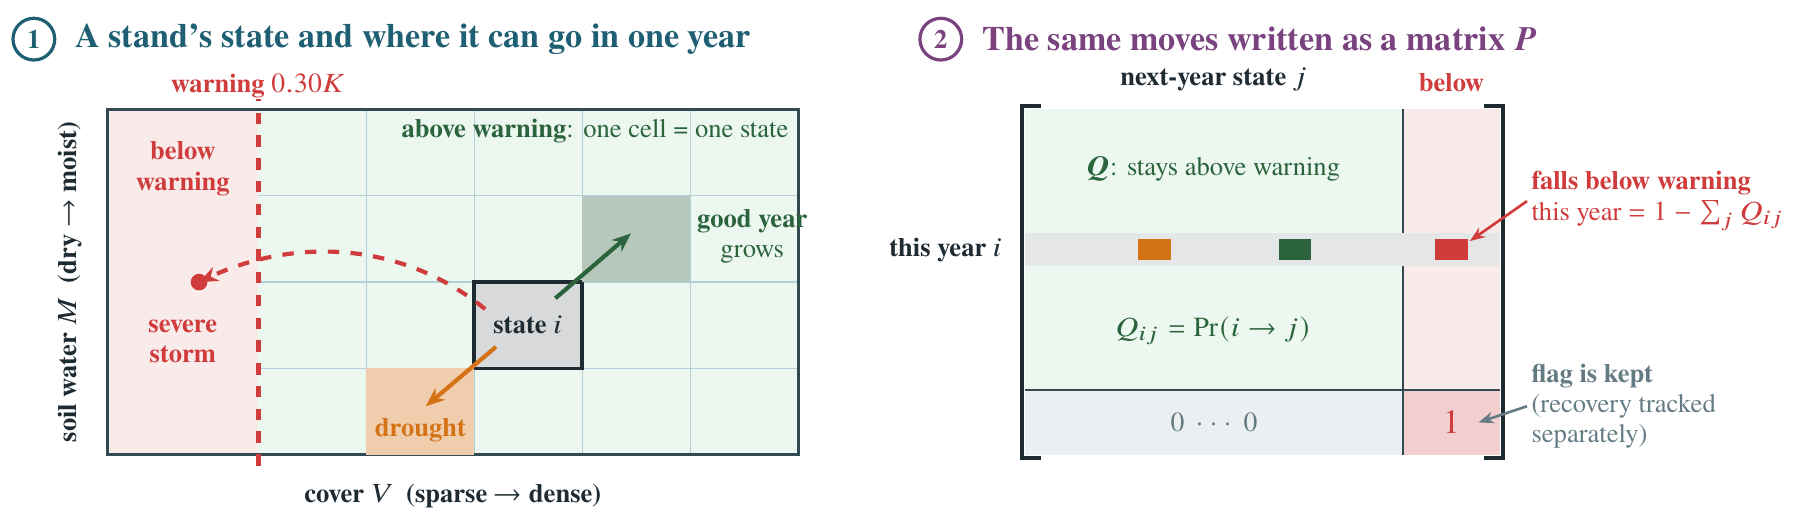
\includegraphics[width=\linewidth]{m3_matrix_discrete.png}
  \caption{Physical meaning of the transition matrix: (1) a stand's state (cover, soil water) and its typical one-year moves; (2) the same moves as one row of $\bm P$.}
  \label{fig:m3-matrix}
\end{figure}

\begin{table}[!htb]
\centering\small
\renewcommand{\arraystretch}{1.05}
\begin{tabularx}{\linewidth}{@{}l X r l@{}}
\toprule
Symbol & Meaning (stress-test scenario, not calibrated) & Base value & Tested \\
\midrule
$\lambda_0;\ U$ & storm rate; cover loss per storm & $0.25$/yr; $\mathrm{U}(0.10,0.50)$ & $3\times3$ grid \\
$p_D;\ \gamma$ & drought probability; storm multiplier in drought & $0.12{+}0.002t;\ 1.5$ & no drought; $\gamma=1$ \\
$\alpha_u,\alpha_R,\alpha_\lambda$ & yearly trends in wind, rain, storm rate & $+0.5\%,-0.5\%,+1\%$ & stationary \\
$\rho,\beta;\ H$ & flag threshold, area share; horizon & $0.30K,\ 50\%;\ 50$\,yr & $0.20K$, $0.40K$ \\
\bottomrule
\end{tabularx}
\caption{Model~3 scenario parameters.}
\label{tab:m3-par}
\end{table}

\subsection{Results}
\paragraph{The belt is hit often but recovers.} Under the baseline stress test, the belt is flagged within 10 years with probability $77.5\%$, and $\mathrm{RMST}(50)=7.1$\,yr. The $600$\,mm/yr core strip B resists more than twice as long ($16.1$\,yr) as cohorts A and C ($7.1$--$7.2$\,yr; Figure~\ref{fig:m3-res}a). A flag, however, is not a collapse: by year~50 almost all $300$\,ha has crossed $0.30K$ at some point, yet only $200$\,ha is below it, so about \textbf{$99$\,ha has recovered} on stored water and continued irrigation (Figure~\ref{fig:m3-res}b). The belt still delivers $4{,}762\text{ effective ha}\cdot\text{yr}$, $65.5\%$ of the disaster-free path (Figure~\ref{fig:m3-res}c). In drought years the canal caps bind from April to September and cut May delivery by $26\%$ (Figure~\ref{fig:m3-res}d).

\begin{figure}[!htb]
  \centering
  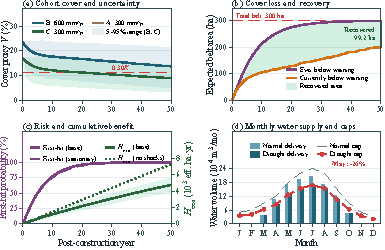
\includegraphics[width=0.96\linewidth]{m3_resilience.pdf}
  \caption{50-year stress test from Model~2's year 15 ($6{,}000$ paths, threshold $0.30K$): (a) cohort cover and 5--95\% path range, (b) ever-crossed vs.\ currently low area, (c) flag probability and cumulative cover, (d) monthly canal supply in normal and drought years.}
  \label{fig:m3-res}
\end{figure}

\paragraph{What drives the risk.} Water and wind responses were already tested in Model~1 and are not repeated. Two post-construction findings remain (Figure~\ref{fig:m3-sens}), and the numerical check confirms them:
\begin{enumerate}\setlength{\itemsep}{1pt}\setlength{\parsep}{0pt}
  \item \textbf{Storm frequency and severity dominate.} $\mathrm{RMST}(50)$ ranges from $41.8$\,yr (rare, mild storms) to $2.8$\,yr (frequent, severe storms); the baseline sits in the high-risk corner (a).
  \item \textbf{More water helps little once canals are full.} Asking for $20\%$ more water raises $\mathrm{RMST}$ only from $7.1$ to $8.1$\,yr because summer caps clip the extra request; removing droughts or the drought--storm link gains less than a year (b).
  \item \textbf{The numbers are numerically reliable.} The Markov chain lies inside the Monte Carlo $95\%$ interval at all 9 check points; refining the grid or the storm nodes changes probabilities by at most $0.04$ and $0.20$ percentage points.
\end{enumerate}

\begin{figure}[!htb]
  \centering
  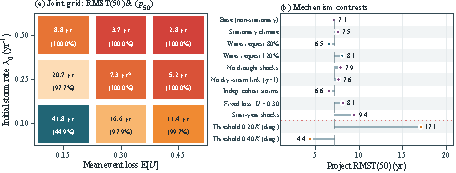
\includegraphics[width=\linewidth]{m3_sensitivity_val.pdf}
  \caption{(a) $\mathrm{RMST}(50)$ and 50-year flag probability over storm rate and loss ($^*$ uses loss range $[0.15,0.45]$); (b) project $\mathrm{RMST}(50)$ under mechanism contrasts.}
  \label{fig:m3-sens}
\end{figure}

\paragraph{Summary.} The planned belt is frequently pushed below the warning level by compound disasters, but most damage is temporary while water keeps flowing. Higher water on core strips and secure dry-summer canal supply matter more than extra annual quota.


\clearpage


% Task 4: an unnumbered, one-page letter to the responsible officials.
\clearpage
\begingroup\small
\setlength{\parindent}{0pt}
\setlength{\parskip}{5pt}
\phantomsection
\addcontentsline{toc}{section}{Policy Letter: Holding the Taklamakan Green Belt}
\label{sec:brief}
{\large\bfseries Holding the Taklamakan Green Belt: A Practical Operating Plan\par}
\vspace{3pt}
\textbf{To:} County officials responsible for forestry, water resources, and project finance\par
Our study of the Yutian--Minfeng section links a 15-year construction and operating plan with a further 50-year disaster stress test. The baseline schedule below offers a practical starting point, conditional on reliable water deliveries, funded maintenance, and viable electricity sales.\par
\textbf{Secure water before expanding.} Confirm monthly deliveries before approving new planting. Baseline May demand reaches 95\% of monthly delivery capacity, making spring supply the immediate bottleneck. Service pumps and drip lines before May; postpone expansion if existing stands lack water and publish drought allocation rules.\par
\textbf{Make maintenance accountable.} Assign each block a supervisor and check survival after planting and the first summer. Increase irrigation as stands mature, check soil moisture before changing deliveries, and correct irrigation faults or burial damage before replanting.\par
\textbf{Fiscal burden} The baseline requires about CNY 44.3 million in planting and PV capital during years 1--4. During years 5--15, modelled annual PV income of CNY 4.1--4.3 million exceeds annual upkeep and water costs of CNY 1.8--2.0 million. We recommend public funding for planting and essential water infrastructure, with the operator responsible for upkeep. Earmark viable PV revenue for maintenance, equipment replacement, and a disaster reserve. Itemise annual costs, review spending quarterly, and secure funding gaps before expansion; these revenues depend on electricity prices and operating conditions.\par
\textbf{Protect communities and report results.} Prioritise vulnerable sections near roads, settlements, and farmland, and include local workers in maintenance contracts. Coordinate irrigation with household and agricultural needs. Publish vegetation condition, water deliveries, spending, and unfinished repairs annually, with a contact for public reports.\par
\textbf{Expected benefits.} Sustained care can maintain shelter near roads, settlements, and farmland while supporting recurring local maintenance work. In the baseline 50-year stress scenario, continued irrigation preserves 65.5\% of the cumulative vegetation-cover benefit of the disaster-free case, showing that damaged stands can still provide substantial long-term value.\par
A comprehensive \textbf{policy chart} would be like:


\vspace{2pt}
\begingroup\footnotesize
\setlength{\tabcolsep}{4pt}\renewcommand{\arraystretch}{1.18}
\begin{tabularx}{\linewidth}{@{}>{\raggedright\arraybackslash}p{0.16\linewidth} >{\raggedright\arraybackslash}X >{\raggedright\arraybackslash}p{0.23\linewidth}@{}}
\toprule
\textbf{When} & \textbf{Practical action} & \textbf{Lead responsibility} \\
\midrule
Years 1--2 & Plant 3 square kilometres of shelterbelt, subject to confirmed water and maintenance funding. & Water authority and planting contractor \\
Years 1--4 & Install 9.5 MW of PV only with grid access, viable returns, and sufficient budget. & Project operator and finance department \\
Years 5--15 & Fund upkeep from operating income; inspect irrigation before May and audit spending quarterly. & Operator and irrigation team \\
Year 16 onward & Continue monitoring and funded upkeep; inspect after droughts or storms and repair recoverable stands. & Monitoring and maintenance teams \\
\bottomrule
\end{tabularx}
\endgroup\par
\textbf{Expected benefits.} Sustained care can maintain shelter near roads, settlements, and farmland while supporting recurring local maintenance work. In the baseline 50-year stress scenario, continued irrigation preserves 65.5\% of the cumulative vegetation-cover benefit of the disaster-free case, showing that damaged stands can still provide substantial long-term value.\par
\vspace{2pt}
Yours sincerely,\\
\textit{The Modelling Team}
\par\endgroup
\clearpage


\clearpage
\begingroup
\renewcommand*{\bibfont}{\small}
\setlength{\bibitemsep}{2pt}
\setlength{\bibparsep}{0pt}
\setlength{\emergencystretch}{3em}
\printbibliography[heading=bibintoc,title={References}]
\endgroup

\end{document}
